\begin{figure*}[t]
  \centering
  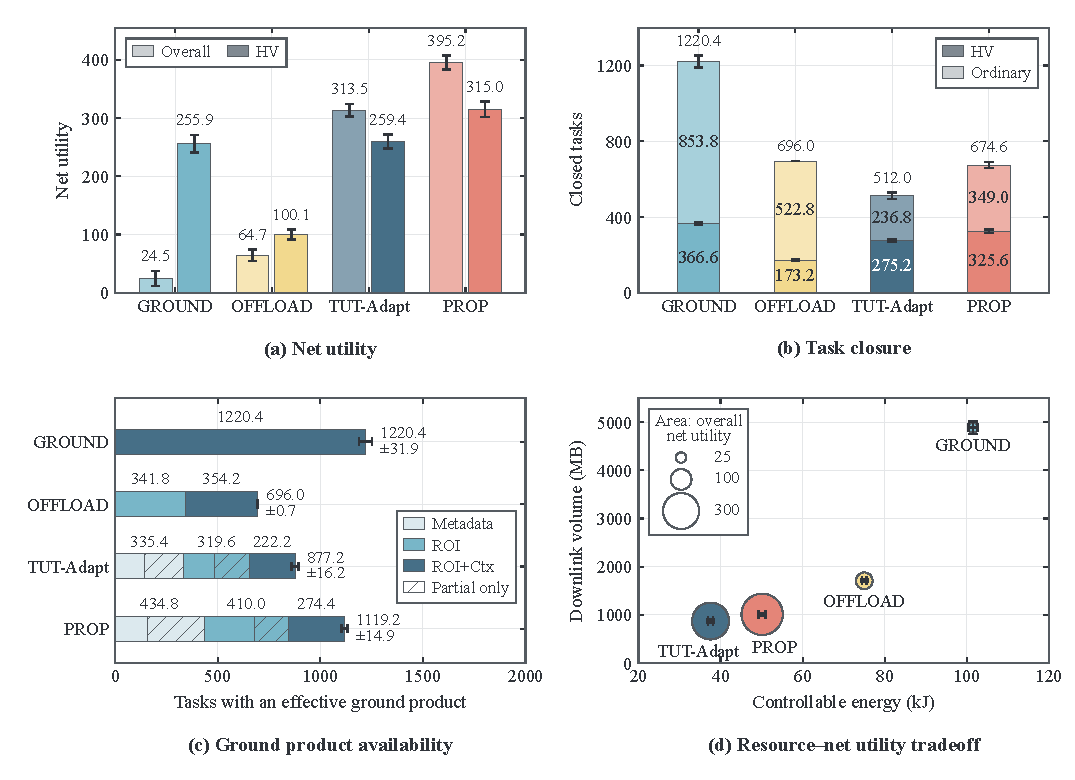
\includegraphics[width=\textwidth]{main_exp.pdf}
  \caption{Main results over five seeds (4101--4105), each with 1,600 tasks (448 high-value, HV) over 6 h. Values are means; error bars and $\pm$ terms denote sample SD (ddof=1). (a) Net utility is realized ground benefit minus fixed public energy, downlink, and queue costs. (b) Error bars indicate HV and total closures. (c) Each task is counted once at its highest valid ground product available within the observation period and before its deadline; solid and hatched portions indicate requirement satisfaction and partial-only delivery, respectively. Labels above bars give product-category totals. (d) Bubble area is proportional to overall net utility; error bars show resource SD. Controllable energy excludes the common 191.376 kJ background load; downlink uses decimal MB. Ground products in (c), including ground-processed results, differ from the actual transmitted payloads measured in (d).}
  \label{fig:main-exp}
\end{figure*}
